\documentclass[
	letterpaper, % Paper size, specify a4paper (A4) or letterpaper (US letter)
	10pt, % Default font size, specify 10pt, 11pt or 12pt
]{CSUniSchoolLabReport}

%----------------------------------------------------------------------------------------
%	REPORT INFORMATION
%----------------------------------------------------------------------------------------

\title{Basics of Signals \\ Circuits \& Signals \\ EECE2150} % Report title

\author{Michael \textsc{Brodskiy}}

\date{February 8, 2023} % Date of the report

%----------------------------------------------------------------------------------------


\begin{document}

\maketitle % Insert the title, author and date using the information specified above

\begin{center}
	\begin{tabular}{l r}
		Date Performed: & January 23, 2023 \\ % Date the experiment was performed
        Partner: & Juan \textsc{Zapata} \\ % Partner names
		Instructor: & Professor \textsc{Sun} % Instructor/supervisor
	\end{tabular}
\end{center}

\setcounter{section}{-1}

\section{Introduction}

The purpose of this laboratory experimentation is to provide an introduction to working and analyzing signals. This lab focuses on frequency and alternating current to lay a foundation for signals.

\section{Frequency}

\subsection{Q1}

\subsubsection{(a)} The sound seems to be proportional to the voltage; that is, it appears to get louder the higher the voltage is

\subsubsection{(b)} A change in frequency seems to affect the pitch of the sound; the higher the frequency, the higher the pitch

\subsection{Q2} The upper frequency bound was approximately $18.8[\si{\kilo\hertz}]$. At this point, both my partner and I stopped hearing the speaker. The lower bound was approximately $31.8[\si{\hertz}]$. At this point, it was too low pitch for my partner and I to hear. Our hearing is fairly close to general human boundaries, but may have been affected by the fact that the speakers were set to a low volume, making it harder to hear while there was lots of background noise in the room. As the frequency gets closer to the middle of the human range, it seems to be the loudest, anywhere from $1[\si{\kilo\hertz}]$ to $13[\si{\kilo\hertz}]$. This is probably that, as humans, we are able to hear in this range the best. The maximum loudness seems to occur at $3.5[\si{\kilo\hertz}]$. Although it could depend on the speaker and its volume, I think this is the best point humans can hear at.

\subsection{Q3} Our group was able to guess the exact pitch, which was $800[\si{\hertz}]$. Though the fact that the answer was a fairly round number made it easier to guess (as opposed to something like 823), it was still a bit difficult to guess. This was done by manipulating our speaker slowly until the sounds seemed to match, or, at least, sound similar.

\subsection{Q6\footnote{Numbering of the questions in the lab was out of order}} Of the three pulse types (triangle, sine, and square), square seems to be consistently the loudest. This is probably because when it is active, it is always at the maximum amplitude, as opposed to the other two, which rise and fall. The ramp/triangle configuration was quieter than the square, but louder than sine. Of all of them, sine seemed the smoothest, while square just seemed loud, and triangle sounded sharp to the ear.

\subsection{Q7} All configurations sound the same at $6[\si{\kilo\hertz}]$, as opposed to $600[\si{\hertz}]$. This effect is most likely similar to that of the blinking LEDs from the previous experiment; the LEDs appeared to stop blinking at a certain frequency, while the sound seems to stop pulsing at a high enough frequency.

\section{Fourier Analysis}

\begin{figure}[h!]
  \centering
  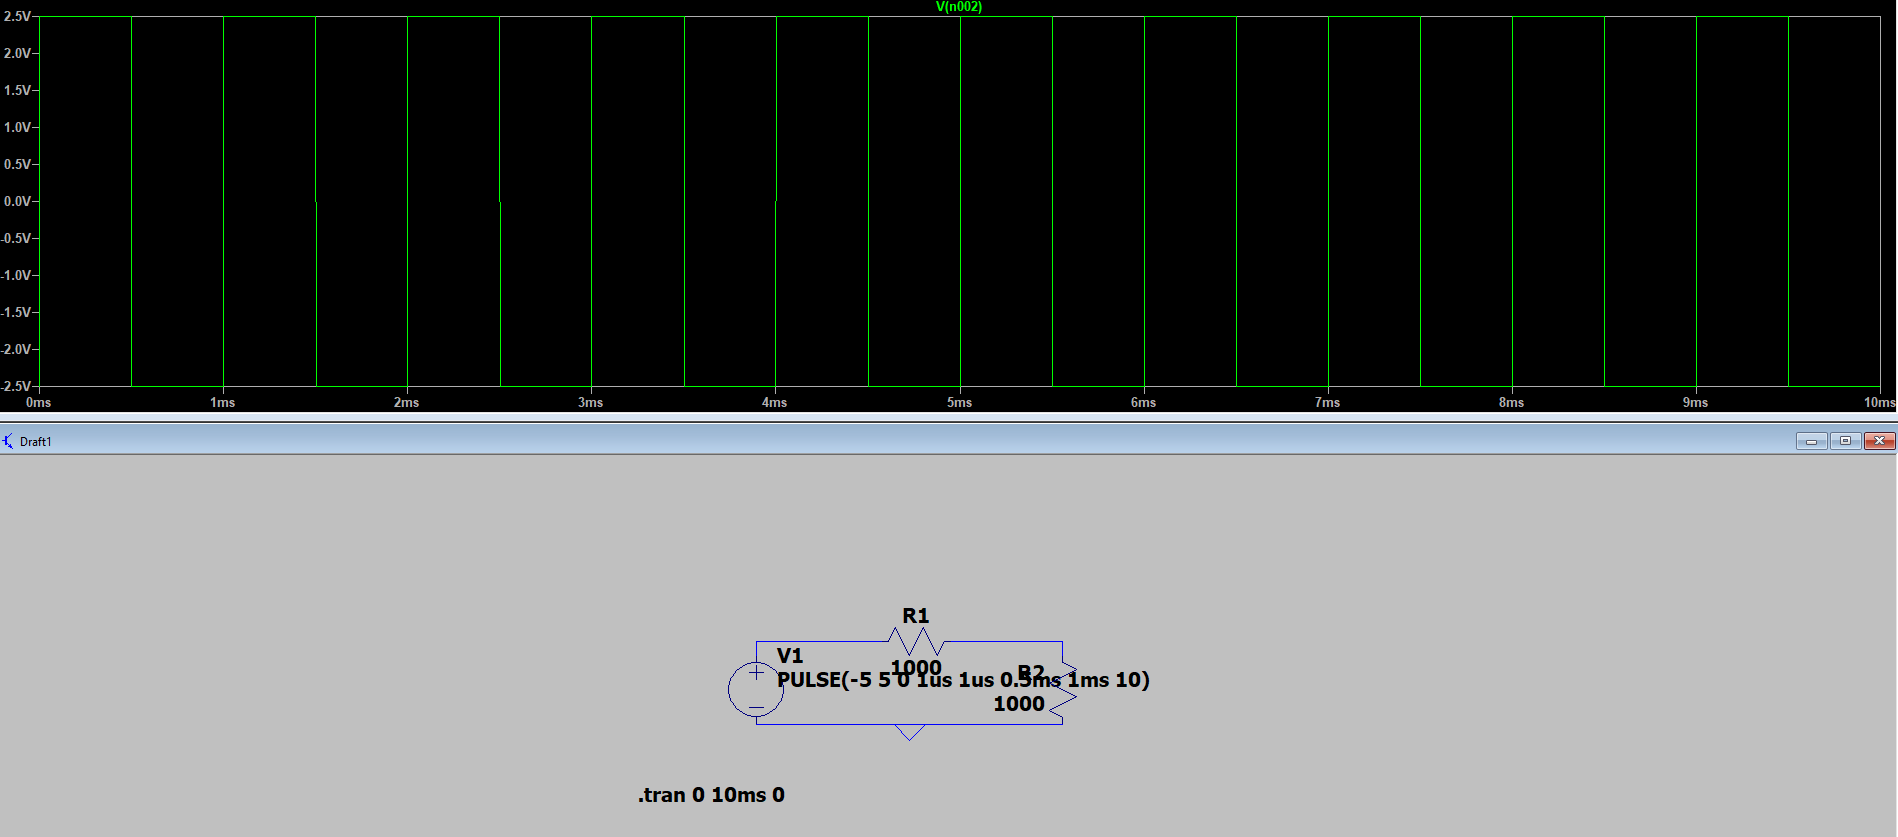
\includegraphics[width=.8\textwidth]{Figures/L4FA1.png}
  \caption{Initial Set-up of the SPICE System}
  \label{fig:1}
\end{figure}

\setcounter{subsection}{2}

\begin{figure}[h!]
  \centering
  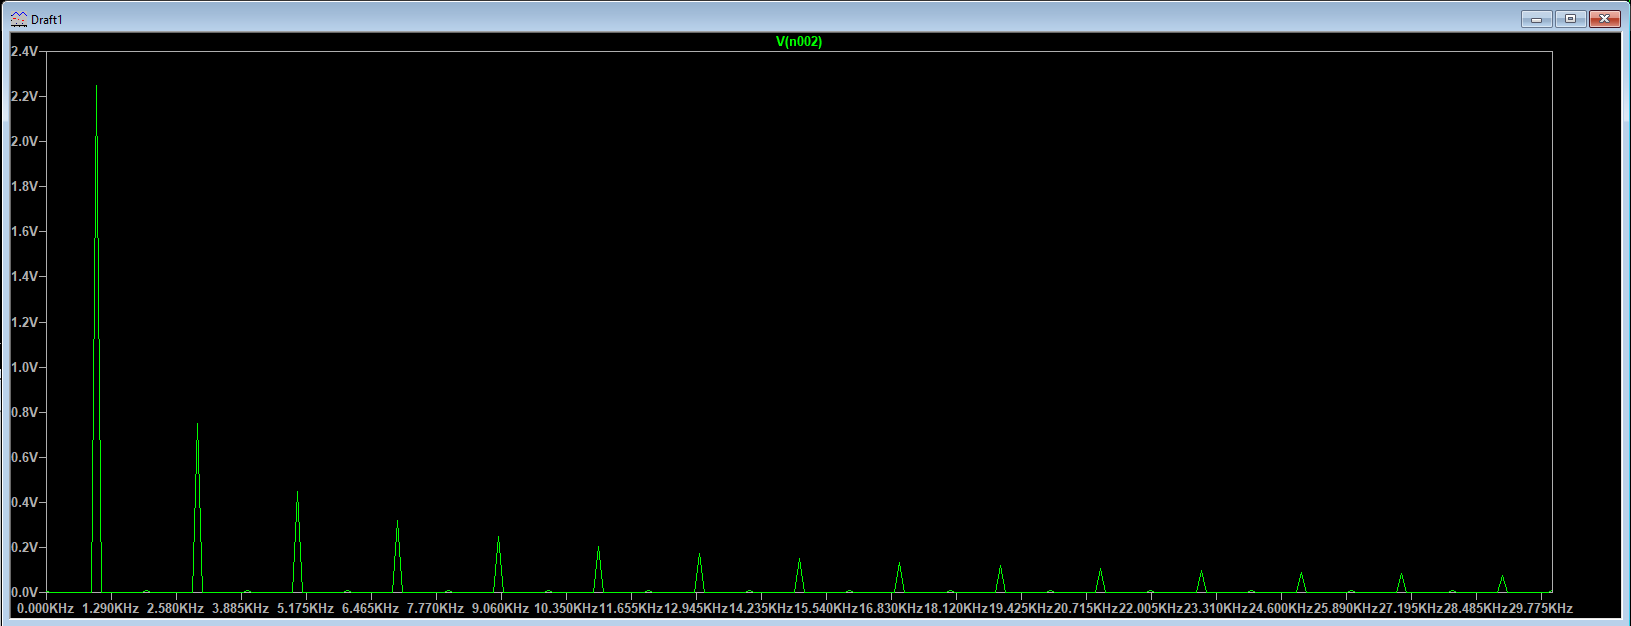
\includegraphics[width=.8\textwidth]{Figures/L4FA2.png}
  \caption{Analysis of $.5[\si{\milli\second}]$ Pulse Width}
  \label{fig:2}
\end{figure}

\begin{figure}[h!]
  \centering
  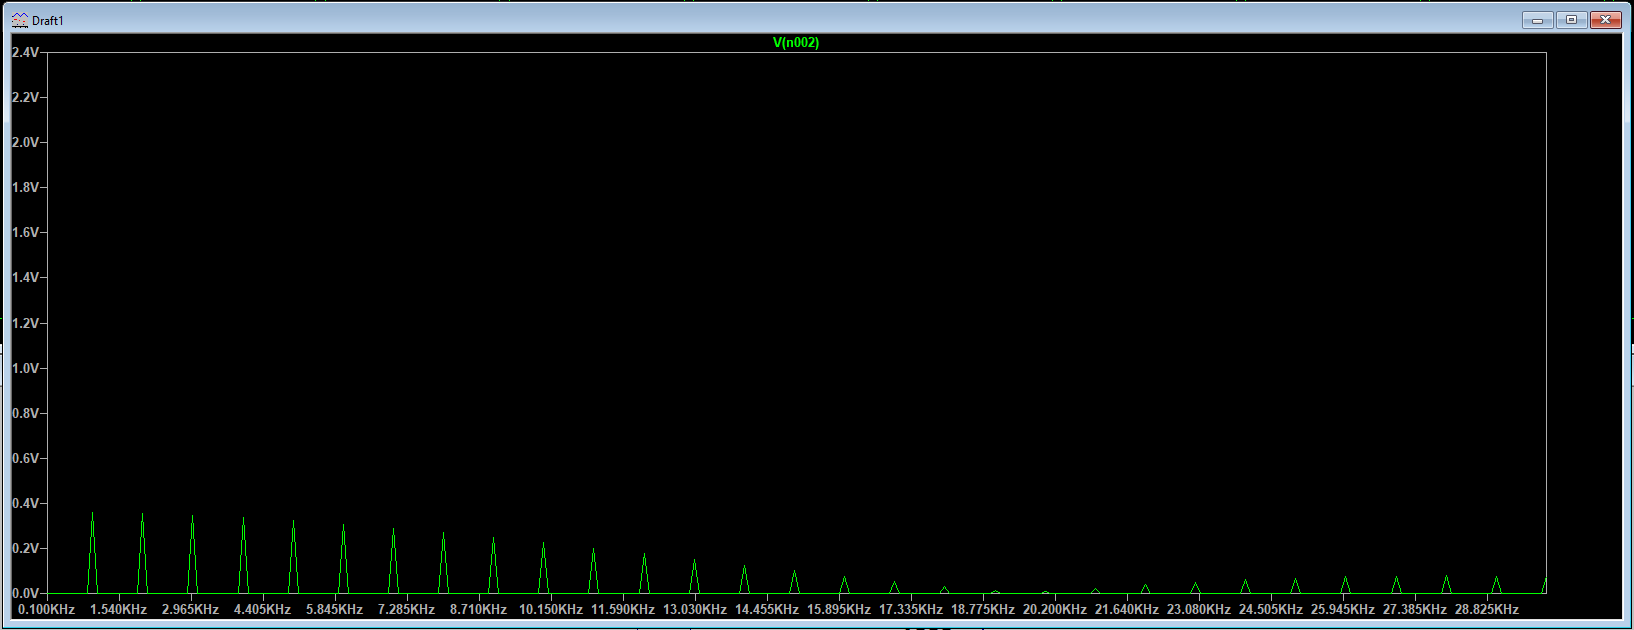
\includegraphics[width=.8\textwidth]{Figures/L4FA3.png}
  \caption{Analysis of $.05[\si{\milli\second}]$ Pulse Width}
  \label{fig:3}
\end{figure}

\subsection{} At a pulse width of $.05[\si{\milli\second}]$, as opposed to $.5[\si{\milli\second}]$, the peaks are shorter. Additionally, the peaks occur more frequently.

\setcounter{subsection}{4}

\begin{figure}[h!]
  \centering
  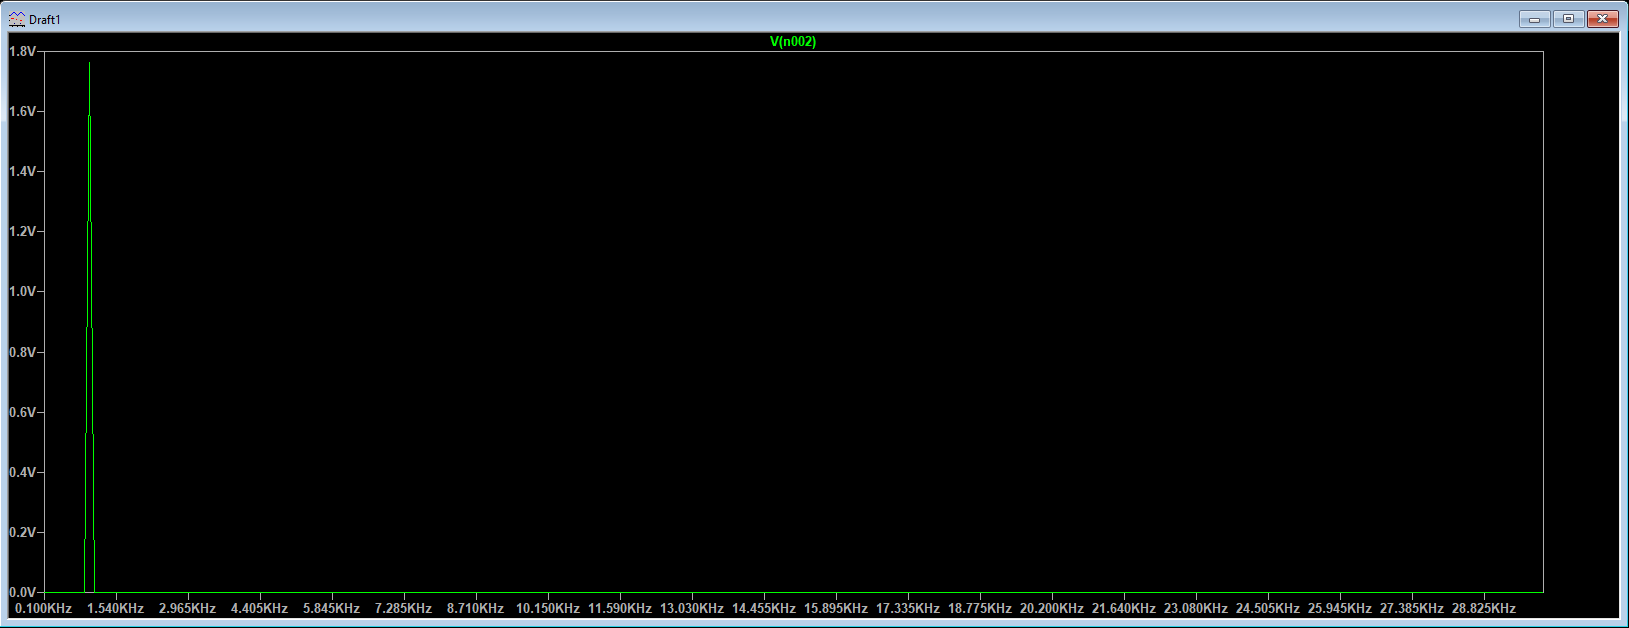
\includegraphics[width=.8\textwidth]{Figures/L4FA4.png}
  \caption{Sinusoidal Wave Transient Analysis}
  \label{fig:4}
\end{figure}

\subsection{} Most likely, the point at which there is a peak for the transient analysis is the only point at which a sine wave could form.

\begin{figure}[h!]
  \centering
  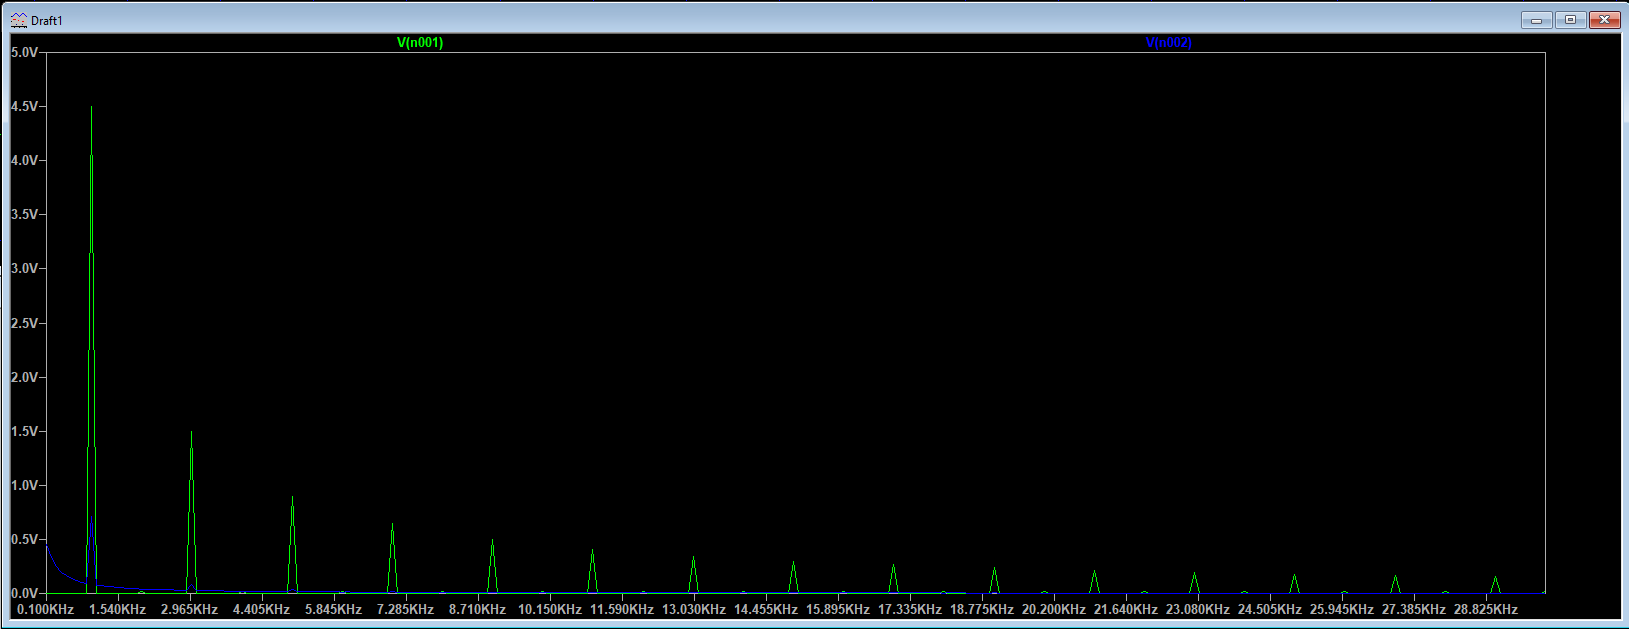
\includegraphics[width=.8\textwidth]{Figures/L4FA5.png}
  \caption{Fourier Analysis of Capacitor}
  \label{fig:5}
\end{figure}

\subsection{} Although the heights of the graphs are actually different, the two voltages have peaks at the same exact frequencies.

\section{Conclusion}

Overall, this laboratory experiment demonstrated the basic concepts of signals, as well as digital tools to analyze them. Though it has not been mathematically defined in the classroom yet, the concept of Fourier and Transient analysis was introduced, which allows for the analysis of AC circuitry.

\end{document}
